% !TEX root =  master.tex
\chapter{Grundlagen }

Um eine wissenschaftliche Grundalge dieser Arbeit zu schaffen, wird zunächst das Thema Pentesting generell betrachtet, in dessen Umfeld sich die Arbeit in der Praxisphase befindet. Dann werden verschiedene Vorgehensweisen und Methoden thematisiert, die zur automatisierten Schwachstellenerkennung verwendet werden. 

\section{Penetration Testing}

Pentration Testing beschreibt den autorisierten und legalen Versuch Computer-Systeme ausfindig zu machen und dessen Schwachstellen erfolgreich auszunutzen, um diese Systeme sicherer zu machen. \\
Der Prozess umfasst sowohl die Identifizierung von Schwachstellen, sowie der Bereitstellung von Proof-of-Concept (POC) Angriffen, um zu demonstrieren, dass die Schwachstellen existent sind. 

Ein ordnungsgemäßer Penetrationtest endet mit einer spezifischen Empfehlung zur Behebung der während des Tests entdeckten Probleme. Insgesamt wird dieser Prozess dazu verwendet, um Computer und Netzwerke gegen zukünftige Angriffe zu sichern. \cite{B1}

Pentester nutzen Tools und Techniken, die auch von böswilligen Angreifern (black hats) verwendet werden, um Schwachstellen in Systemen und Netzwerken zu finden. Dies beinhaltet unter anderem die Überprüfung von Passwortschutz, Netzwerksicherheit und Anwendungssicherheit. \cite{B1}

Darüber hinaus ist Pentesting ein wichtiger Teil des Risikomanagement-Prozesses, da es Unternehmen ermöglicht, ihre Systeme auf potenzielle Bedrohungen zu überprüfen und Gegenmaßnahmen zu ergreifen, bevor Angriffe stattfinden. Jedoch handelt es sich beim Pentesting um eine simulative Übung und bietet daher keine Garantie für die tatsächliche Sicherheit eines Systems. \cite{8}

\subsection{Pentesting Frameworks}

Um bei einem Penetration Test erfolgreiche Ergebnisse 
Bei einem Penetration Test spielt die Methodik eine entschediden 
Ohne die Verwendung einer festen Methodik

Beim Penetration Testing spielt eine gut definierte Methodik eine Schlüsselrolle beim Erreichen von erfolgreichen Ergebnissen. Diese Ergebnisse werden sind jedoch entscheidend um Daten, Anwendungen und die zugrunde legende Infrastruktur zu schützen.
Ohne ein etablierte Methodik während der Durchführung eines Pentests, kann es schwierig sein Lokalisieren von Schwachstellen schwierig sein oder sogar ein falsches Sicherheitsgefühl der Anwendung erwecken. \\
Nach Willhelm P. sind Penetration Tests Projekte, welche durch effektive, wiederholbare und qualitätssteigenderen Prozessen durchgeführt werden sollten, um dadurch die Qualität dieser Tests deutlich anzuheben. \\
Hierbei spielt die Verwendung einer festgelegten Methodik eine wesentliche Rolle.

\subsection{Standards und Vorgehensweisen}

Wie die meisten Prozesse kann auch ein Penetration Test in einzelne Schritte heruntergebrochen werden. 
Um möglichst effektive Ergebnisse zu garantieren, halten sich die meisten Pentester Standards und Vorgehensweisen, die eine systematische Überprüfung von Systemen erleichtern. 

Je nach Detailorientiertheit wird ein Pentration Test daher in vier bis sieben Schritte eingeteilt. 
Patrick Engebretson unterteilt die Methodik eines Penetrationstests in vier grundlegende Schritte: \cite{B1} 

Der erste Schritt beschreibt die Reconnaissance, also das Sammeln von Informationen und Auskundschaften eines Systems. Hierbei wird zunächst versucht jede mögliche Information über eine System zu erhalten und abzuspeichern. Die in dieser Phase gesammelten Informationen sind für den weiteren Verlauf des Penetrationtests entscheidend. \cite{B1}\\
Man unterscheidet dabei zwischen aktiver und passiver Reconnaissance.
Bei der aktiven Reconnaissance wird direkt mit dem Zielsystem interagiert, um bestimmte Informationen zu erhalten. Hierbei werden aktiv Anfragen an das Zielsystem gesendet. Dabei ist nicht auszuschließen, dass das Zielsystem durch die aktive Reconnaissance alarmiert wird. \\
Bei der passiven Reconnaissance wird nicht aktiv mit dem Zielsystem interagiert. Hierbei werden öffentliche Inhalt verwendet, um Informationen über das Ziel zu sammeln. Das Zielsystem wird dabei nicht alarmiert. \cite{B1} \cite{B4}


\begin{figure}[H]
	\centering
	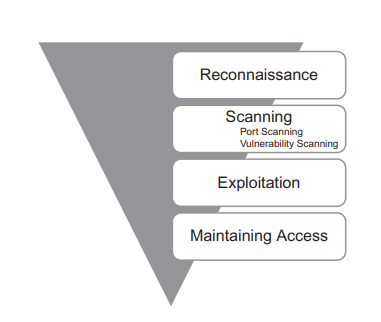
\includegraphics[scale=1]{\imagedir/Phasen_eines_Pentests.png}
	\caption{Phasen eines Penetrationtests}
	\label{Phasen eines Penetrationtests} \cite{B1}
\end{figure}

Das in der Abbildung 1.1 abgebildete Dreieck symbolisiert dabei, dass eine breit angesammelte Menge an Informationen kombiniert mit der passenden Abstraktion über die weiteren Phasen schließlich zu einem erfolgreichen Pentest führt. 

Der zweite Schritt, das Scanning, kann in zwei weitere Bestandteile aufgeteilt werden. Mit den in der Reconnaissance herausgefundenen IP-Adressen kann nun ein Port-Scan durchgeführt werden, um offene Ports und potentielle Services zu identifizieren. \cite{B2} \\
Als nächstes wird das Vulnerability Scanning ausgeführt. Dabei werden Schwachstellen in der Software und in den Services des Zielsystems lokalisiert und identifiziert. \cite{B3}

!! Den Text hier unten nochmal durchchecken, der ist später dazu gekommen !!

Anhand der Ergebnisse unserer Scans können wir nun mit der Exploitation-Phase, also der Ausnutzung von Schwachstellen beginnen. 
Da wir nun genau wissen welche Ports und Services Angriffsfläche bieten und sogar die Schwachstellen kennen, können wir nun beginnen unser Zielsystem systematisch anzugreifen. \cite{B1}\\
Beim exploiting gibt es zahlreiche Ansätze und Vorgehensweisen. Hauptziel ist jedoch immer, Zugriff auf das Zielsystem zu erlangen und seine Zugriffsrechte auf dem System so zu eskalieren, dass man Administratorrechte auf dem Zielsystem erlangt. \cite{B4}

Die letzte Phase die durchschritten wird ist die Maintaining Access Phase. Haufig wird bei einer Ausnutzung einer Schwachstellen nur temporärer Zugriff auf das Zielsystem möglich. \\
Da viele Sicherheitslücken keinen dauerhaften Zugriff erlauben, wird während des temporären Zugriffs im Zielsystem versucht, eine weiter Möglichkeit zu schaffen auf das Zielsystem zu gelangen. \cite{6}

Formal wird einem Pentest in der Regel noch eine letzte Phase, das Reporting hinzugefügt, an welchem oftmals die Qualität eines Pentests gemessen wird.
Ein Report beinhaltete alle relevanten Informationen über den vollzogenen Pentest. 
Hierbei werden Sicherheitslücken aufgedeckt und an den nötigen Stellen wird zusätzlich erläutert, welche Schritte im Pentest stattgefunden haben. 
Gegebenenfalls werden vom Pentester noch Vorschläge gemacht, wie die Sicherheitslücken ausgebessert werden können. \cite{B1}

\section{XY}

Weiterer wissenschaftlicher Input zu Schwachstellen in Web Applikationen z.B. OWASP top 10


